\begin{chapter}{Fault Attacks}
  \begin{boxH}
    \textbf{Fault attacks} consist in \textbf{injecting} malicious \textbf{faults} into the
    \textbf{target device}, aimed at bringing it into a \textbf{set of states} from which private
    internal information items (e.g., a key) can be fraudulently extracted.
  \end{boxH}
  Faults can be either \textit{temporary} or \textit{permanent}, by changing the state of a memory
  address or a register forever.\\
  They idea is pretty simple: take the case of a encryption algorithm, if i run it and get a 1, by
  running that again injecting a fault, we are able to understand what the original bit was. In a
  more formal way, if $C_{\text{OK}}=E(P)$ and $C_{\text{Fault}}=E(P)$ while injecting a fault, for
  example a '0', if $C_{\text{OK}} \neq C_{\text{Fault}}$, then the bit is 0, otherwise it is 1.\\
  This is because we know the memory configuration when the fault is injected, and we can compare 
  the two results.

  \begin{boxH}
    Fault injections \textbf{doesn't} necessary \textbf{require physical} access to the chip, they
    can be performed fully remotely.
  \end{boxH}

  There are many ways to induce a fault in a system, some of them are:
  \begin{itemize}
    \item Underpowering or overvolting the device
    \item altering the clock
    \item changing the temperature
    \item injecting a laser in the device, depackaging it beforehand and shining the laser on the
      silicon (\textit{laser injection})
    \item electromagnetic injections
  \end{itemize}

  By injecting the system with faults, it is possible to achieve many interesting results, like:
  \begin{itemize}
    \item \textbf{bypassing} the \textbf{security} checks
    \item generate \textbf{faulty outputs}, like wrong encrypted messages
    \item generate \textbf{denial of service}
  \end{itemize}
  
  \begin{section}{ Differential Fault Analysis}

    \begin{boxH}
      With \textbf{Differential Fault Analysis} (DFA) \textbf{set} of \textbf{multiple injections}
      with subsequent correlated analysis of the faulty behavior of the target device.
    \end{boxH}
    Here is a simple example of how DFA works: the attackers (cryptanalysts) focus on the fault
    influences of specific hardware implementations to collect some faulty outputs.\\
      Later, this information is compared and analyzed with correct results to harvest some partial
      or total compromise of the secret information.
  \end{section}

  \begin{section}{Fault Injections Countermeasures}
    Several approaches have been proposed, including:
    \begin{itemize}
      \item Preventing the attack
      \item Detecting the fault injection
      \item Detecting the fault effect (error)
      \item De-synchronization
      \item Robust package, “hardened” technologies
    \end{itemize}

    \begin{subsection}{Fault Detection}
      One basic defense system is to \textbf{detect} when the \textbf{attack} is happening, by using
      some kind of \textbf{sensors}, which are connected to the root of trust. The problem with this
      approach false positives in very noisy environments, and even in ideal conditions, attacks are
      still possible to some degree.
    \end{subsection}

    \begin{subsection}{Error Detection}
      Another approach is still based on detection, but we introduce redundancy in the system to
      detect when an error is happening. The redundancy can be multiple execution or inverting the
      operation, for example. Detection is not a very effective mechanism because it is not possible
      to tell which result is the faulty one, and which is the correct one.\\
      Many standards cover fault, eg. fault tolerant systems, and thus they can be used to be a
      valuable countermeasure against fault attacks.\\ 
      In any case, error detection techniques applies to the system some degree of overhead.\\
      In the error detection schema is presented in the figure \ref{fig:error_detection}. The idea
      is that the original stuff is carrying out an operation, and the result is compared to a
      prediction about the output, which can be a safe code. If the two results are different, then
      the system is in error, and we should be able, in some case to recover from the error. This is
      not always possible though, because the more we would like to be able to correct the bigger is
      the code, and thus the overhead.
      \begin{figure}[H]
        \centering
        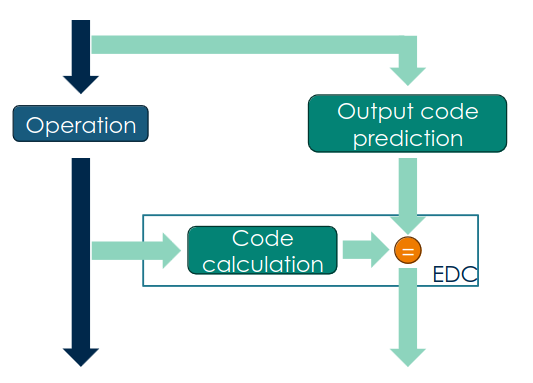
\includegraphics[width=0.5\textwidth]{img/hardware/error detection.png}
        \caption{Error Detection}
        \label{fig:error_detection}
      \end{figure}
      \end{subsection}

      \begin{subsection}{De-synchronization}
        Most of the time fault injects require synchronization, because not all them are permanent.
        If the attacker need a specific timing to inject the fault at the right location, we can
        jitter at a different time, the fault would never appear because the memory has been
        overwritten, and thus the fault would only appear on data that have been already used.
        This is done trough different mechanisms:
        \begin{itemize}
          \item jitter clock
          \item dummy instructions
          \item random operation flow
        \end{itemize}

      \end{subsection}
      \begin{subsection}{Hardened IC Package}
        Another solution is to make an hardened package, because that's the portion that would be
        removed to perform some kinds of injections, because its the component that would have
        protected the chip from the environment.

      \end{subsection}
    \end{section}

  \end{chapter}
